%
% chapter.tex -- Homologie
%
% (c) 2021 Prof Dr Andreas Müller, Hochschule Rapperswil
%
\chapter{Homologie
\label{buch:chapter:homologie}}
\lhead{Homologie}
\rhead{}
Mit der Inzidenzmatrix war es möglich, einen Graphen zu beschreiben
und verschiedene interessante Eigenschaften desselben zu berechnen.
Damit können aber nur eindimensionale Strukturen analysiert werden:
Es ist zum Beispiel nicht möglich, ein Dreieck vom Rand eines
Dreiecks zu unterscheiden~\ref{buch:homologie:figure:zusammenziehbar}.
\begin{figure}
\centering
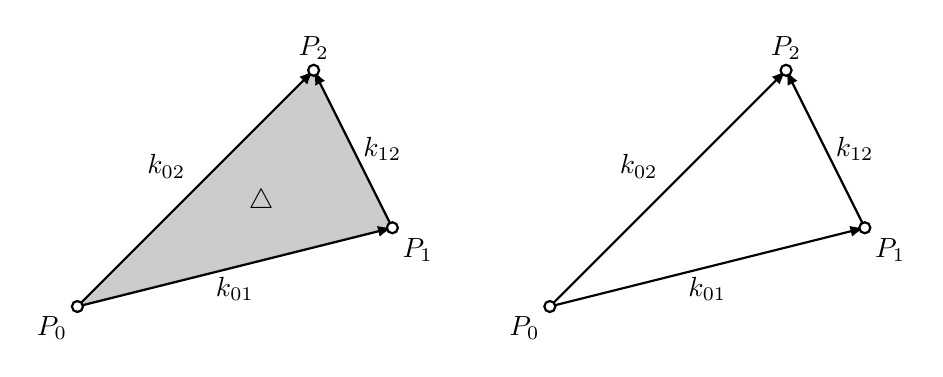
\begin{tikzpicture}[>=latex,thick]
\def\punkt#1{
	\fill[color=white] #1 circle[radius=0.07];
	\draw #1 circle[radius=0.07];
}
\begin{scope}[xshift=3cm]
\draw[->] (0,0) -- (3,3);
\draw[->] (0,0) -- (4,1);
\draw[->] (4,1) -- (3,3);
\node at (0,0) [below left] {$P_0$};
\node at (4,1) [below right] {$P_1$};
\node at (3,3) [above] {$P_2$};
\punkt{(0,0)}
\punkt{(4,1)}
\punkt{(3,3)}
\node at (2,0.5) [below] {$k_{01}$};
\node at (1.5,1.5) [above left] {$k_{02}$};
\node at (3.5,2) [right] {$k_{12}$};
\end{scope}
\begin{scope}[xshift=-3cm]
\fill[color=gray!40] (0,0) -- (4,1) -- (3,3) -- cycle;
\draw[->] (0,0) -- (3,3);
\draw[->] (0,0) -- (4,1);
\draw[->] (4,1) -- (3,3);
\node at (0,0) [below left] {$P_0$};
\node at (4,1) [below right] {$P_1$};
\node at (3,3) [above] {$P_2$};
\node at (2,0.5) [below] {$k_{01}$};
\node at (1.5,1.5) [above left] {$k_{02}$};
\node at (3.5,2) [right] {$k_{12}$};
\node at (2.333,1.333) {$\triangle$};
\punkt{(0,0)}
\punkt{(4,1)}
\punkt{(3,3)}
\end{scope}
\end{tikzpicture}
\caption{Ein Dreieck $\triangle$ (rechts) und der Rand des Dreicks
(links) sind mit den Methoden
der Graphentheorie nicht unterschiedbar. 
Als topologische Räume sind das Dreieck und sein Rand aber ganz klar
unterschiedbar: In einem Dreieck ist jeder geschlossene Pfad in einen 
Punkt zusammenziehbar, aber die Randkurve ist nicht mehrzusammenziehbar,
sobald man das innere des Dreiecks entfernt.
\label{buch:homologie:figure:zusammenziehbar}}
\end{figure}
Die Randkurve ist in einem Dreieck zusammenziehbar, aber sobald man
das innere des Dreiecks entfernt, ist die Randkurve nicht mehr
zusammenziehbar.
Dreieck und der Rand des Dreiecks sind also grundsätzlich verschieden.

Die Inzidenzmatrix ordnet jeder Kante ihre beiden Endpunkte zu.
Die Homologietheorie verallgemeinert diese Idee.
Der sogenannte Randoperator ordnet jedem Dreieck, Tetraeder oder allgemein
jedem Simplex seinen Rand zu.
Damit wird es möglich, das Dreieck vom Rand des Dreiecks zu unterschieden.

%
% simplex.tex -- simplizes und Polyeder
%
% (c) 2021 Prof Dr Andreas Müller, OST Ostschweizer Fachhochschule
%
\section{Simplizes
\label{buch:section:simplexe}}
\rhead{Simplizes}
Die Idee, das Dreieck und seinen Rand zu unterscheiden verlangt,
dass wir zunächst Dreiecke und deren höherdimensionale Verallgemeinerungen,
die sogenannten Simplizes entwickeln müssen.

\subsection{Simplizes und Rand
\label{buch:subsection:simplices}}
Die Inzidenz-Matrix eines Graphen hat einer Kante die beiden Endpunkte
mit verschiedenen Vorzeichen zugeordnet.

\subsubsection{Rand eines Dreiecks}
Dieses Idee soll jetzt verallgemeinert werden.
Der Rand des Dreiecks $\triangle$ in
Abbildung~\ref{buch:homologie:figure:zusammenziehbar}
besteht aus den Kanten $P_0P_1$, $P_1P_2$ und $P_0P_2$.
Für eine algebraische Definition müssen die Kanten offenbar eine
Orientierung haben, die ist aber garantiert, da wir den Anfangs-
und Endpunkten einer Kante verschiedene Vorzeichen gegeben haben.
Dem Dreieck $\triangle$ werden dann die drei Kanten $k_{01}$, $k_{02}$
und $k_{12}$ zuogeordnet, aber mit zusätzlichen Vorzeichen, die
die Orientierung festhalten.
Durchläuft man den Rand von $\triangle$ in der Reihenfolge $P_0P_1P_2$,
dann müssen die Kanten $k_{12}$ und $k_{02}$ ein negatives Vorzeichen
erhalten.

Wir können diese Zuordnung wieder mit einer Matrix ausdrücken.
\[
\begin{matrix}
\text{$k_{01}$:}\mathstrut\\
\text{$k_{02}$:}\mathstrut\\
\text{$k_{12}$:}\mathstrut
\end{matrix}
\qquad
\partial
=
\begin{pmatrix*}[r]
1\mathstrut\\
-1\mathstrut\\
1\mathstrut
\end{pmatrix*}
\]

\subsubsection{Standardsimplizes}
Punkte, Kanten und Dreiecke sind die einfachsten Fälle sogenannter
Simplizes.
Wir formulieren die Definition dieser Objekte auf eine Weise,
die uns ermöglichen soll, sie auf beliebige Dimension zu verallgemeinern.

Die Strecke, die die Punkte $P$ und $Q$ miteinander verbindet,
kann beschrieben werden durch eine Parametrisierung
der Form
\begin{equation}
s_1
\colon
t
\mapsto
t\vec{p} + (1-t) \vec{q}
=
t_0 \vec{p} + t_1\vec{q},
\end{equation}
wobei die beiden positiven reellen Zahlen $t_0,t_1\in\mathbb{R}$ die
Bedingung $t_0 + t_1 = 1$ erfüllen.
Für ein eindimensionales Objekt brauchen wir also zwei Punkte und zwei
positive Parameter, die sich zu $1$ summieren.
Die Mengen $\triangle_1=\{ (t_0,t_1)\,|t_i\ge 0, t_0+t_1=1\}$ kann also
ganz allgemein als Parameterraum zur Beschreibung eindimensionalen Objektes
mit den Endpunkten dienen.
Eine Strecke ist also eine Abbildung der Form
\begin{equation}
s_1
\colon
\triangle_1 \to \mathbb{R}^N
:
(t_0,t_1)
\mapsto
t_0 \vec{p} + t_1\vec{q},
\end{equation}
und der Rand besteht aus den Punkten $s_1(0)$ und $s_1(1)$, wobei der
Anfangspunkt $s_1(0)$ mit einem negativen Vorzeichen versehen wird.

Für höhere Dimensionen brauchen wir auf analoge Weise erst wieder einen
geeigneten Parameterraum.
Die Menge
\begin{equation}
\triangle_n
=
\{(t_0,\dots,t_n)\in\mathbb{R}^{n+1}\mid t_i\ge 0,t_0+t_1+\dots+t_n=1\}
\subset\mathbb{R}^{n+1}
\label{buch:homologie:eqn:standardsimplex}
\end{equation}
beschreibt zum Beispiel für $n=2$ ein Dreieck und für $n=3$ ein 
Tetraeder.
\index{Tetraeder}%

\begin{definition}
Die Menge $\triangle_n$ von \eqref{buch:homologie:eqn:standardsimplex}
heisst das $n$-dimensionale Standardsimplex.
\index{Standardsimplex}%
\end{definition}

Die Standardbasisvektoren von  $\mathbb{R}^{n+1}$ werden $e_0,\dots,e_n$
bezeichnet und sind die Ecken des $n$-dimensionalen Standardsimplex.

\subsubsection{Simplizes in $\mathbb{R}^N$}
Gegeben $n+1$-Punkte $P_0,\dots,P_n$ mit Ortsvektoren
$\vec{p}_0,\dots,\vec{p}_n\in\mathbb{R}^N$, können wir eine Abbildung
\begin{equation}
s_n
\colon
\triangle_n
\to
\mathbb{R}^N
:
(t_0,\dots,t_n)
\mapsto
t_0\vec{p}_0
+
t_1\vec{p}_1
+
\dots
+
t_n\vec{p}_n
\end{equation}
Eine solche Abbildung verallgemeinert also den Begriff einer Strecke
in einem Raum $\mathbb{R}^N$  
auf höhere Dimensionen.
Sie ist durch die Eckpunkte vollständig vorgegeben, es reicht also
die Punkte $P_0,\dots,P_n\in\mathbb{R}^N$ zu kennen.

%\begin{definition}
%\label{buch:def:simplex}
%Ein $n$-dimensionales {\em Simplex} oder {\em $n$-Simplex} in $X$ ist eine
%stetige Abbildung $s_n\colon\triangle_n\to X$.
%\end{definition}
%
%Die Ecken des $n$-Simplex $\triangle_n$ sind die Standardbasisvektoren
%in $\mathbb{R}^{n+1}$.
%Mit $e_k$ bezeichnen wird die Ecke, deren Koordinaten $t_i=0$ sind für 
%$k\ne i$, ausser der Koordinaten $t_k$, die den Wert $t_k=1$ hat.


\begin{definition}
Ein $n$-Simplex in $\mathbb{R}^N$ ist die stückweise lineare Abbildung
$s\colon \triangle_n\to \mathbb{R}^N$ gegeben durch die Bilder der Eckpunkte
$P_i = s(e_i)$.
Wir schreiben auch $[P_0,P_1,\dots,P_n]$ für dieses Simplex.
\end{definition}

\subsubsection{Rechnen mit Simplizes}
Wir möchten später ein geometrisches Objekt aus Simplizes zusammensetzen.
Dazu müssen wir mehrere Simplizes so ein einen Raum abbilden können, dass
sie an den Rändern zusammenpassen.
Dazu müssen wir mit ``Kombinationen'' von Simplizes rechnen können.
Wir betrachten daher
jedes Simplex als einen Basisvektor eines abstrakten Vektorraumes.

Simplizes verschiedener Dimension in $\mathbb{R}^N$ können natürlich 
immer unterschieden werden, wir können also den Vektorraum in einzelne
Vektorräume aufteilnen, einen für jede Dimension.
In Dimension $l$ bezeichnen wir mit $C_l$ den Vektorraum, dessen
Basisvektoren $l+1$-Tupel
\(
[P_0,\dots,P_l]
\)
von Punkten von $\mathbb{R}^N$ sind.
Der Vektorraum $C_l$ besteht dann aus Linearkombinationen
\[
C_l
=
\biggl\{
\sum x_{P_0\dots P_l} [P_0,\dots,P_l]
\;\bigg|\;
x_{P_0\dots P_l}\in\mathbb{R}
\biggr\}.
\]
Die Seitenflächen dieses Simplex sind die $l-1$-dimensionalen
Simplizes, die man erhält, indem man eine Ecke weglässt.
Wir bezeichnen mit $[P_0,\dots,\widehat{P_i},\dots,P_l] \in C_{l-1}$
Die Seitenfläche, die man durch Weglassen der Ecke $P_i$
erhalten hat.

\subsubsection{Rand eines Simplex}
Die Oberfläche eines Simplex ist nicht einfach die Summe der
Seitenflächen.
Die Kanten eines Dreiecks $[P_0,P_1,P_2]$ müssen so aneinandergefügt
werden, dass sie einen Weg um das Dreieck ergeben.
Beginnt man das Dreieck in Richtung der Kanten
$[P_0,P_1]$ und $[P_1,P_2]$ zu umlaufen, trifft man in
``verkehrter'' Richtung auf die Kante $[P_0,P_2]$.
Für den Rand des Dreiecks muss man also diese Kante mit negativem
Vorzeichen zählen:
\begin{align*}
\partial_3 \colon
[P_0,P_1,P_2]
\mapsto
[P_0,P_1]
+ [P_1,P_2]
- [P_0,P_2]
&=
[\widehat{P_0},P_1,P_2]
-[P_0,\widehat{P_1},P_2]
+[P_0,P_1,\widehat{P_2}]
\\
&=
\sum_{i=0}^l (-1)^i [P_0,\dots,\widehat{P_i},\dots,P_3]
\end{align*}
Dies ist auch die Art, wie Kanten des Dreiecks $\triangle$ 
in Abbildung~\ref{buch:homologie:figure:zusammenziehbar}
orientiert wurden.

\begin{definition}
\label{buch:def:randoperator}
Der Randoperator ordnet einem $l$-Simplex dessen $l-1$-dimensonale
Seitenflächen mit alternierenden Vorzeichen zu:
\[
\partial_l : [P_0,\dots,P_l]
\mapsto
\sum_{i=0}^l (-1)^i [P_0,\dots,\widehat{P_i},\dots,P_l].
\]
\end{definition}

\subsubsection{Inzidenzmatrix eines gerichteten Graphen und Randoperator}
In Abschnitt~\ref{buch:graphen:subsection:inzidenzmatrix} wurde die
Inzidenzmatrix eines gerichteten Graphen $G=(V,E)$ definiert.
Seien $V=\{v_1,\dots,v_n\}$ die Vertizes des Graphen und
$E=\{e_1,\dots,e_m\}$ die Kanten. 
Gibt es eine Kante $e_k = (v_i,v_j)\in E$ im Graphen, dann hat die Inzidenzmatrix
in Spalte $k$ die Einträge $-1$ in Zeile $i$ und $+1$ in Zeile $j$.
Die Kante $e_k$ können wir als eindimensionales Simplex $[v_i,v_j]$
betrachten.
Die Adjazenzmatrix ordnet ihm die Linearkombination
\[
A(G)\colon e_k=[v_i,v_j] \mapsto -[v_i] +[v_j]
= (-1)^0 [\widehat{v_i},v_j] + (-1)^1 [v_i,\widehat{v_j}]
=
\partial_2 [v_i,v_j]
\]
zu.
Die Adjazenzmatrix eines Graphen kann man also als den Randoperator
$\partial_1$ betrachten, der auf den als $1$-dimensionale Simplizes
betrachteten Kanten des Graphen wirkt.

\subsubsection{Der Rand des Randes}
Der Rand eines Tetraeders setzt sich aus vier Dreiecken
zusammen.
Jede Kante gehört zu genau zwei Seitenflächen. 
Wenn die Dreiecke alle so orientiert sind, dass sie ``von ausserhalb''
des Tetraeders betrachtet positiv orientiert sind, dann wird jede
Kante zweimal in jeder Richtung durchlaufen.
Bildet man den Rand all dieser Seitenflächen, kommte jede Kante
einmal mit positivem und einmal mit negativem Vorzeichen vor,
die Summe ist $0$.

Ganz allgemein gilt, dass der Rand des Randes verschwindet.

\begin{satz}
\label{buch:homologie:satz:randrand}
Es gilt $\partial_{l-1}\circ\partial_l=0$.
\end{satz}

\begin{proof}[Beweis]
Der Rand des Simplex $[P_0,\dots,P_l]$ ist
\[
\partial_l[P_0,\dots,P_l]
=
\sum_{i=0}^l (-1)^i [P_0,\dots,\widehat{P_i},\dots,P_l].
\]
Darauf muss jetzt der Randoperator $\partial_{l-1}$ angewendet
werden.
Dabei wird jeweils der Index $i$ übersprungen, bei der Bildung der
Summe müssen die Teile daher separat betrachtet werden:
\begin{align}
\partial_{l-1}\partial_l[P_0,\dots,P_l]
&=
\sum_{i=0}^l (-1)^i \partial_{l-1}[P_0,\dots,\widehat{P_i},\dots,P_l]
\notag
\\
&=
\sum_{i=0}^l (-1)^i
\biggl(
\sum_{j<i} (-1)^j
[P_0,\dots,\widehat{P_j},\dots,\widehat{P_i}\dots,P_l]
\notag
\\
&\hspace*{2cm}
+
\sum_{j>i} (-1)^{j-1}
[P_0,\dots,\widehat{P_i},\dots,\widehat{P_j}\dots,P_l]
\biggr)
\label{buch:homologie:eqn:randrand}
\\
&=
\sum_{j<i} (-1)^{i+j}
[P_0,\dots,\widehat{P_j},\dots,\widehat{P_i}\dots,P_l]
-
\sum_{j>i} (-1)^{i+j}
[P_0,\dots,\widehat{P_i},\dots,\widehat{P_j}\dots,P_l]
\notag
\end{align}
Der Exponent $j-1$ im zweiten Term von
\eqref{buch:homologie:eqn:randrand}
trägt der Tatsache Rechnung,
dass der Index $i$ übersprungen worden ist.
In der zweiten Summe kann man die Summationsindizes umbenennen,
also $i$ durch $j$ ersetzen und umgekehrt, dann entsteht
\begin{align*}
\partial_{l-1}\partial_l[P_0,\dots,P_l]
&=
\sum_{j<i} (-1)^{i+j}
[P_0,\dots,\widehat{P_j},\dots,\widehat{P_i}\dots,P_l]
\\
&\qquad
-
\sum_{i>j} (-1)^{j+i}
[P_0,\dots,\widehat{P_j},\dots,\widehat{P_i}\dots,P_l]
\\
&=0.
\qedhere
\end{align*}
\end{proof}

\subsection{Polyeder}
\begin{figure}
\centering
\includegraphics{chapters/95-homologie/images/polyeder.pdf}
\caption{Aufbau eines zweidimensionalen Polyeders aus
verschiedenen Simplizes.
Die Schnittmenge zweier Simplizes muss ein Untersimplex beider Simplizes
sein.
Die roten Kreise im linken Bild weisen auf verschiedene Situationen
hin, wo das diese Bedingung nicht erfüllt ist.
In rechten Bild sind zusätzliche Simlizes hinzugefügt worden, um
die Bedingungen eines Polyeders zu erfüllen.
\label{buch:homologie:figure:polyeder}}
\end{figure}
Aus einzelnen Simplizes können jetzt kompliziertere geometrische
Objekte gebaut werden.
Ein Graph ist ein Beispiel für ein geometrisches Objekt, welches
als Vereinigung von 1-Simplizes entsteht.
Die Vereinigung ist aber nicht beliebig, vielmehr ist die Schnittmenge
zweier beliebiger 1-Simplizes immer entweder leer, eine Menge 
mit nur einem Vertex oder ein ganzes 1-Simplex.

Für höhere Dimensionen muss diese Idee ausgedehnt werden auf
höherdimensionale Simplizes.
In einem Graphen dürfen sich Kanten nicht in einem inneren Punkt treffen,
sondern nur in Endpunkten.
Verallgemeinert auf höherdimensionale Simplizes kann man dies als die
Bedingung formulieren, dass die Schnittmenge zweier beliebiger
Simplizes immer Untersimplizes beider Simplizes sein müssen.
Wir fassen dies zusammen in der folgenden Definition.

\begin{definition}
\index{Polyeder}%
\index{Dimension eines Polyeders}%
\index{Polyeder, Dimension eines}%
Ein {\em Polyeder} ist eine Vereingung von endlich vielen Simplizes derart,
dass die Schnittmenge zweier beliebiger Simplizes immer ein Untersimplex
beider Simplizes ist.
Die {\em Dimension} des Polyeders ist die grösste Dimension der darin
enthaltenen Simplizes.
\end{definition}

Ein Graph ist nach dieser Definition ein eindimensionales Polyeder.
Die Mengen in der Abbildung~\ref{buch:homologie:figure:polyeder}
ist kein Polyeder, kann aber leicht zu einem Polyeder gemacht werden,
indem man einzelne Kanten mit zusätzlichen Punkten unterteilt.
Auch müssen die zweidimensionalen Simplizes aufgeteilt werden.

Abbildung~\ref{buch:homologie:figure:polyeder} zeigt auch, dass
die Darstellung einer Punktmenge als Polyeder nicht eindeutig ist.
Man kann die Kanten und Flächen jederzeit weiter unterteilen, ohne
dass sich die Gestalt der gesamten Menge dadurch ändert.

\subsection{Triangulation
\label{buch:subsection:triangulation}}
Unser Ziel ist, geometrische Objekte besser verstehen zu können.
Dabei sind uns Deformationen und sogar Knicke egal, es interessiert uns
nur die ``Gestalt'' des Objekts.
Entfernungen zwischen Punkten sind ebenfalls von untergeordneter 
Bedeutung, da sie bei Deformation nicht erhalten bleiben.
Der Begriff des ``topologischen Raumes'' fasst diese Ideen mathematisch
präzise ein, eine genaue Definition würde aber an dieser Stelle zu weit
führen.
Stattdessen beschränken wir uns auf eine Klasse von Punktmengen, die man
mit Simplizes beschreiben kann.

Ein topologischer Raum zeichnet sich durch einen Nachbarschaftsbegriff
von Punkte aus, der erlaubt zu definieren, was eine stetige Abbildung ist.
Ein stetige Abbildungen bildet nahe beeinander liegende Punkte wieder
auf nahe beeinander liegende Punkte ab.
Dass nahe liegende Punkte nicht plötzlich auf weit auseinander liegende
Punkte abgebildet werden gibt die Intuition wieder, dass Deformationen
möglich sein sollen, dass der Raum dabei aber nicht ``reissen'' darf.
Zwei topologische Räume $X$ und $Y$ können daher als ``gleichgestaltig''
betrachtet werden, wenn es zwei stetige Abbildungen $f\colon X\to Y$
und $g\colon Y\to X$ gibt, die zu einander invers sein.
Oder wenn sich $X$ stetig auf $Y$ abbilden lässt, so dass auch die
Umkehrabbildung stetig ist.
Eine solche Abbildung heisst ein {\em Homöomorphismus}, die beiden Räume
$X$ und $Y$ heissen {\em homomorph}.

Eine Kugel ist natürlich kein Polyeder, aber sie kann leicht homöomorph
auf ein dreidimensionales Simplex abgebildet werden.

\begin{beispiel}
Sei $T$ ein reguläres Tetraeder mit den Ecken auf der dreidimensionalen
Einheitskugel $B^3$.
Für jeden Richtungsvektor $x\ne 0$ sei $l(x)$ Entfernung vom Mittelpunkt des
Tetraeders bis zum Durchstosspunkt einer Geraden durch den Mittelpunkt
mit Richtungsvektor $x$ durch die Oberfläche des Tetraeders.
Dann sind die Abbildungen
\[
f\colon
T\to B^3
:
x \mapsto\begin{cases}
\displaystyle
\frac{x}{l(x)}&\quad\text{für $x\ne 0$}\\
0&\quad\text{für $x=0$}
\end{cases}
\qquad\text{und}\qquad
g\colon
B^3\to T
:
x \mapsto\begin{cases}
l(x) x&\quad\text{für $x\ne 0$}\\
0&\quad\text{für $x=0$}
\end{cases}
\]
zueinander inverse stetige Abbildungen oder Homöomorphismen.
\end{beispiel}

Im Folgenden sollen daher nur solche topologischen Räume untersucht werden,
die homöomorph sind zu einem Polyeder.
Man nennt die homöomorphe Abbildung eines Polyeders auf so einen Raum
auch eine Triangulation.
Durch Unterteilung der Simplizes in kleiner Simplizes kann eine solche
Triangulation beliebig verfeinert werden.







%
% komplex.tex -- komplexe Zahlen
%
% (c) 2021 Prof Dr Andreas Müller, OST Ostschweizer Fachhochschule
%
\section{Komplexe Zahlen
\label{buch:section:komplexe-zahlen}}
\rhead{Komplexe Zahlen}
In den reellen Zahlen lassen sich viele algebraische Gleichungen lösen,
die in $\mathbb{Q}$ nicht lösbar waren.
Andere, z.~B.~die Gleichung
\begin{equation}
x^2+1=0,
\label{buch:zahlen:eqn:igleichung}
\end{equation}
haben weiterhin keine Lösung.
Der Grund dafür ist das Bestreben bei der Konstruktion der reellen Zahlen, 
die Ordnungsrelation zu erhalten.
\index{Ordnungsrelation}%
Diese ermöglicht, Näherungsintervall und Intervallschachtelungen
zu definieren.

Die Ordnungsrelation sagt aber auch, dass $x^2\ge 0$ ist für jedes
$x\in\mathbb{R}$, so dass $x^2+1>0$ sein muss.
Dies ist der Grund, warum die Gleichung \ref{buch:zahlen:eqn:igleichung}
keine Lösung in $\mathbb{R}$ haben kann.
Im Umkehrschluss folgt auch, dass eine Erweiterung der reellen Zahlen,
in der die Gleichung \eqref{buch:zahlen:eqn:igleichung} lösbar ist,
ohne die Ordnungsrelation auskommen muss.
Es muss darin Zahlen geben, deren Quadrat negativ ist und der
Grössenvergleich dieser Zahlen untereinander ist nur eingeschränkt
möglich.

\subsubsection{Imaginäre und komplexe Zahlen}
Den reellen Zahlen fehlen also Zahlen, deren Quadrat negativ ist.
Nach inzwischen bewährtem Muster konstruieren wird die neuen Zahlen
daher als Paare $(a,b)$.
Die erste Komponente soll die bekannten reellen Zahlen darstellen,
deren Quadrat positiv ist.
Die zweite Komponente soll für die Zahlen verwendet werden, deren Quadrat
negativ ist.
Die Zahl, deren Quadrat $-1$ sein soll, bezeichnen wir mit dem
Paar $(0,1)$ und schreiben dafür auch $i=(0,1)$ mit $i^2=-1$.
Das Paar $i=(0,1)$ heisst auch die {\em imaginäre Einheit}.
\index{imaginäre Einheit}%

Die Rechenregeln sollen weiterhin erhalten bleiben, sie müssen daher
wie folgt definiert werden:
\begin{equation}
\begin{aligned}
(a,b) + (c,d) &= (a+c,b+d) &&& (a+bi) + (c+di) &= (a+c) + (b+d)i
\\
(a,b) \cdot (c,d) &= (ad-bd, ad+bc) &&& (a+bi)\cdot(c+di) &= ac-bd + (ad+bc)i.
\end{aligned}
\label{buch:zahlen:cregeln}
\end{equation}
Diese Regeln ergeben sich ganz natürlich aus den Rechenregeln
in $\mathbb{R}$ unter Berücksichtigung der Regel $i^2=-1$.

Eine komplexe Zahl ist ein solches Paar, die Menge der komplexen Zahlen
ist
\[
\mathbb{C}
=
\{a+bi\;|\;a,b\in\mathbb{R}\}
\]
mit den Rechenoperationen~\eqref{buch:zahlen:cregeln}.
Die Menge $\mathbb{C}$ verhält sich daher wie eine zweidimensionaler
reeller Vektorraum.

\subsubsection{Real- und Imaginärteil}
Ist $z=a+bi$ eine komplexe Zahl, dann heisst $a$ der {\em Realteil} $a=\Re z$
\index{Realteil}%
und $b$ heisst der {\em Imaginärteil} $\Im z$.
\index{Imaginärteil}%
Real- und Imaginärteil sind lineare Abbildungen $\mathbb{C}\to\mathbb{R}$,
sie projizieren einen Punkt auf die Koordinatenachsen, die entsprechend
auch die reelle und die imaginäre Achse heissen.

Die Multiplikation mit $i$ vertauscht Real- und Imaginärteil:
\[
\Re (iz)
=
-b
=
-\Im z
\qquad\text{und}\qquad
\Im (iz)
=
a
=
\Re z.
\]
Zusätzlich kehrt das Vorzeichen der einen Komponente.
Wir kommen auf diese Eigenschaft zurück, wenn wir später in
Abschnitt~\ref{buch:grundlagen:subsection:ringe}
komplexe Zahlen als Matrizen beschreiben.

\subsubsection{Gausssche Zahlenebene}
Beschränkt man die Multiplikation auf einen reellen Faktor, wird $\mathbb{C}$
zu einem zweidimensionalen reellen Vektorraum.
Man kann die komplexe Zahl $a+bi$ daher auch als Punkt $(a,b)$ in der
sogenannten {\em Gaussschen Ebene} betrachten (Abbildung~\ref{buch:zahlen:cfig}).
\index{Gaussche Zahlenebene}%
Die Addition von komplexen Zahlen ist in diesem Bild die vektorielle
Addition, die Multiplikation mit reellen Zahlen werden wir weiter unten
genauer untersuchen müssen.

\begin{figure}
\centering
\includegraphics{chapters/05-zahlen/images/komplex.pdf}
\caption{Argument und Betrag einer komplexen Zahl $z=a+ib$ in der 
Gaussschen Zahlenebene
\label{buch:zahlen:cfig}}
\end{figure}%

Die Zahlenebene führt auf eine weitere mögliche Parametrisierung einer
komplexen Zahl.
Ein Punkt $z$ der Ebene kann in Polarkoordinaten auch durch den {\em Betrag}
\index{Betrag}%
\index{Polarkoordinaten}%
und den Winkel zwischen der reellen Achse und dem Radiusvektor zum Punkt,
dem sogenannten {\em Argument},
charakterisiert werden.

\subsubsection{Komplexe Konjugation}
Der komplexen Zahl $u=a+bi$ ordnen wir die sogenannte
{\em komplex konjugierte} Zahl $\overline{z} = a-bi$.
Mit Hilfe der komplexen Konjugation kann man den Real- und Imaginärteil
\index{komplexe Konjugation}%
\index{Konjugation, komplexe}%
algebraisch ausdrücken:
\[
\Re z 
=
\frac{z+\overline{z}}2
=
\frac{a+bi+a-bi}{2}
=
\frac{2a}2
=a
\qquad\text{und}\qquad
\Im z
=
\frac{z-\overline{z}}{2i}
=
\frac{a+bi-a+bi}{2i}
=
\frac{2bi}{2i}
=
b.
\]
In der Gaussschen Zahlenebene ist die komplexe Konjugation eine
Spiegelung an der reellen Achse.

\subsubsection{Betrag}
In $\mathbb{R}$ kann man die Ordnungsrelation dazu verwenden zu entscheiden,
ob eine Zahl $0$ ist. 
Wenn $x\ge 0$ ist und $x\le 0$, dann ist $x=0$.
In $\mathbb{C}$ steht diese Ordnungsrelation nicht mehr zur Verfügung.
Eine komplexe Zahl ist von $0$ verschieden, wenn die Länge des Vektors in der
Zahlenebene verschieden von $0$ ist.
Wir definieren daher den {\em Betrag} einer komplexen Zahl $z=a+bi$ als
\index{Betrag}
\[
|z|^2
=
a^2 +b^2
=
(\Re z)^2 + (\Im z)^2
\qquad\Rightarrow\qquad
|z|
=
\sqrt{a^2+b^2}
=
\sqrt{(\Re z)^2 + (\Im z)^2}.
\]
Der Betrag lässt sich auch mit Hilfe der komplexen Konjugation ausdrücken,
es ist $z\overline{z} = (a+bi)(a-bi) = a^2+abi-abi+b^2 = |z|^2$.
Der Betrag ist immer eine reelle Zahl.

\subsubsection{Division}
Die Erweiterung zu den komplexen Zahlen muss auch die Division erhalten.
Dies ist durchaus nicht selbstverständlich.
Man kann zeigen, dass ein Produkt von Vektoren eines Vektorraums nur für
einige wenige, niedrige Dimensionen überhaupt möglich ist.
Für die Division sind die Einschränkungen noch gravierender, die einzigen
Dimensionen $>1$, in denen ein Produkt mit einer Division definiert werden
kann\footnote{Der Beweis dieser Aussage ist ziemlich schwierig und wurde
erst im 20.~Jahrhundert mit Hilfe der Methoden der algebraischen Topologie
erbracht. Eine Übersicht über den Beweis kann in Kapitel~10 von
\cite{buch:ebbinghaus} gefunden werden.}, sind $2$, $4$ und $8$.
Nur in Dimension $2$ ist ein kommutatives Produkt möglich, dies muss das
Produkt der komplexen Zahlen sein.

Wie berechnet man den Quotienten $\frac{z}{w}$ für zwei beliebige komplexe
Zahlen $z=a+bi$ und $w=c+di$ mit $w\ne 0$?
Dazu erweitert man den Bruch mit der komplex Konjugierten des Nenners:
\begin{align*}
\frac{z}{w}
&=
\frac{z\overline{w}}{w\overline{w}}
=
\frac{z\overline{w}}{|w|^2}
\end{align*}
Da der Nenner $|w|^2>0$ eine reelle Zahl ist, ist die Division einfach,
es ist die Multiplikation mit der reellen Zahl $1/|w|^2$.

Wir können den Quotienten auch durch Real- und Imaginärteil ausdrücken:
\begin{align*}
\frac{z}{w}
&=
\frac{a+bi}{c+di}
=
\frac{(a+bi)(c+di)}{(c+di)(c-di)}
=
\frac{ac-bd +(ad+bc)i}{c^2+d^2}.
\end{align*}


\subsubsection{Geometrische Interpretation der Rechenoperationen}
Die Addition komplexer Zahlen wurde bereits als Vektoraddition
in der Gausschen Zahlenebene interpretiert. 
Die Multiplikation ist etwas komplizierter, wir berechnen Betrag
und Argument von $zw$ separat.
Für den Betrag erhalten wir
\begin{align*}
|zw|^2
&=
zw\overline{(zw)}
=
zw\overline{z}\overline{w}
=
z\overline{z}w\overline{w}
=
|z|^2|w|^2
\end{align*}
Der Betrag des Produktes ist also das Produkt der Beträge.

Für das Argument verwenden wir, dass
\[
\tan\operatorname{arg}z
=
\frac{\Im z}{\Re z}
=
\frac{b}{a}
\qquad\Rightarrow\qquad
b=a\tan\operatorname{arg}z
\]
und analog für $w$.
Bei der Berechnung des Produktes behandeln wir nur den Fall $a\ne 0$ 
und $c\ne 0$, was uns ermöglicht, den Bruch durch $ac$ zu kürzen:
\begin{align*}
\tan\arg wz
&=
\frac{\Im wz}{\Re wz}
=
\frac{ad+bc}{ac-bd}
=
\frac{\frac{d}{c} + \frac{b}{a}}{1-\frac{b}{a}\frac{d}{c}}
=
\frac{
\tan\operatorname{arg}z+\tan\operatorname{arg}w
}{
1+
\tan\operatorname{arg}z\cdot\tan\operatorname{arg}w
}
=
\tan\bigl(
\operatorname{arg}z+\operatorname{arg}w
\bigr).
\end{align*}
Im letzten Schritt haben wir die Additionsformel für den Tangens verwendet.
\index{Additionstheorem für Tangens}%
Daraus liest man ab, dass das Argument eines Produkts die Summe der
Argumente ist.
Die Multiplikation mit einer festen komplexen Zahl führt also mit der ganzen
komplexen Ebene eine Drehstreckung durch.
Auf diese geometrische Beschreibung der Multiplikation werden wir zurückkommen,
wenn wir die komplexen Zahlen als Matrizen beschreiben wollen.

\subsubsection{Algebraische Vollständigkeit}
Die komplexen Zahlen $\mathbb{C}$ sind als Erweiterung von $\mathbb{R}$
so konstruiert worden, dass die Gleichung $x^2+1=0$ eine Lösung hat.
Etwas überraschend ist dagegen, dass in dieser Erweiterung jetzt jede
beliebige algebraische Gleichung lösbar geworden ist.
Dies ist der Inhalt des Fundamentalsatzes der Algebra.

\begin{satz}[Fundamentalsatz der Algebra]
\label{buch:zahlen:satz:fundamentalsatz}
\index{Fundamentalsatz der Algebra}%
Jede algebraische Gleichung der Form
\[
p(x)=x^n + a_{n-1}x^{n-1}+a_1x+a_0=0,\qquad a_k\in\mathbb{C}
\]
mit komplexen Koeffizienten hat $n$ möglicherweise mit Vielfachheit
gezählte Nullstellen $\alpha_1,\dots,\alpha_m$, d.~h.~das Polynom $p(x)$
lässt sich in Linearfaktoren
\[
p(x)
=
(x-\alpha_1)^{k_1}(x-\alpha_2)^{k_2}\cdot\ldots\cdot(x-\alpha_m)^{k_m}
\]
zerlegen, wobei $k_1+k_2+\dots+k_m=n$.
Die Zahl $k_j$ heisst die {\em Vielfachheit} der Nullstelle $\alpha_j$.
\end{satz}

Der Fundamentalsatz der Algebra wurde erstmals von Carl Friedrich Gauss
\index{Gauss, Carl Friedrich}%
vollständig bewiesen.
Seither sind viele alternative Beweise mit Methoden aus den verschiedensten
Gebieten der Mathematik gegeben worden.
Etwas salopp könnten man sagen, dass der Fundamentalsatz ausdrückt, dass
die Konstruktion der Zahlensysteme mit $\mathbb{C}$ abgeschlossen ist,
soweit damit die Lösbarkeit beliebiger Gleichungen angestrebt ist.

\subsubsection{Quaternionen und Octonionen}
Die komplexen Zahlen ermöglichen eine sehr effiziente Beschreibung 
geometrischer Abbildungen wie Translationen, Spiegelungen und 
Drehstreckungen in der Ebene.
Es drängt sich damit die Frage auf, ob sich $\mathbb{C}$ so erweitern
lässt, dass man damit auch Drehungen im dreidimensionalen Raum
beschreiben könnte.
Da Drehungen um verschiedene Achsen nicht vertauschen, kann eine solche
Erweiterung nicht mehr kommutativ sein.

William Rowan Hamilton propagierte ab 1843 eine Erweiterung von $\mathbb{C}$
\index{Hamilton, William Rowan}%
mit zwei zusätzlichen Einheiten $j$ und $k$ mit den nichtkommutativen
Relationen
\begin{equation}
i^2 = j^2 = k^2 = i\!jk = -1.
\label{buch:zahlen:eqn:quaternionenregeln}
\end{equation}
Er nannte die Menge aller Linearkombinationen 
\[
\mathbb{H} = \{ a_0+a_1i+a_2j+a_3k\;|\; a_l\in \mathbb{R}\}
\]
die {\em Quaternionen}, die Einheiten $i$, $j$ und $k$ heissen auch
\index{Quaternionen}%
Einheitsquaternionen.
\index{Einheitsquaternionen}%
Konjugation, Betrag und Division können ganz ähnlich wie bei den
\index{Konjugation von Quaternionen}%
\index{Betrag einer Quaternion}%
\index{Division durch eine Quaternion}%
komplexen Zahlen definiert werden und machen $\mathbb{H}$ zu einer
sogenannten {\em Divisionsalgebra}.
\index{Divisionsalgebra}%
Alle Rechenregeln mit Ausnahme der Kommutativität der Multiplikation
sind weiterhin gültig und durch jede von $0$ verschiedene Quaternion
kann auch dividiert werden.

Aus den Regeln für die Quadrate der Einheiten in
\eqref{buch:zahlen:eqn:quaternionenregeln} folgt zum Beispiel
$i^{-1}=-i$, $j^{-1}=-j$ und $k^{-1}=-k$.
Die letzte Bedingung liefert daraus
\[
i\!jk=-1
\qquad\Rightarrow\qquad
\left\{
\quad
\begin{aligned}
i\!j
&=
i\!jkk^{-1}=-1k^{-1}=k
\\
i^2\!jk&=-i=-jk
\\
-j^2k&=-ji=k
\end{aligned}
\right.
\]
Aus den Relationen~\eqref{buch:zahlen:eqn:quaternionenregeln}
folgt also insbesondere auch, dass $i\!j=-ji$.
Ebenso kann abgeleitet werden, dass $jk=-k\!j$ und $ik=-ki$.
Man sagt, die Einheiten sind {\em antikommutativ}.
\index{antikommutativ}%

Die Beschreibung von Drehungen mit Quaternionen ist in der
Computergraphik sehr beliebt, weil eine Quaternion mit nur vier
Komponenten $a_0,\dots,a_3$ vollständig beschrieben ist.
Eine Transformationsmatrix des dreidimensionalen Raumes enthält
dagegen neun Koeffizienten, die vergleichsweise komplizierte 
Abhängigkeiten erfüllen müssen.
Kapitel~\ref{chapter:clifford} behandelt nicht nur die Beschreibung
von Drehungen des dreidimensionalen Raumes sondern eine weitreichende
Verallgemeinerung dieser Idee, die sogenannte {\em geometrische Algebra}.
\index{geometrische Algebra}%
Quaternionen haben auch in weiteren Gebieten interessante Anwendungen,
zum Beispiel in der Quantenmechanik, wo antikommutierende Operatoren
\index{Quantenmechanik}%
bei der Beschreibung von Fermionen eine zentrale Rolle spielen.
\index{Fermion}%

Aus rein algebraischer Sicht kann man die Frage stellen, ob es eventuell
auch noch grössere Divisionsalgebren gibt, die $\mathbb{H}$ erweitern.
Tatsächlich hat Arthur Cayley 1845 eine achtdimensionale Algebra,
die Oktonionen $\mathbb{O}$, mit vier weiteren Einheiten beschrieben.
\index{Cayley, Arthur}%
Allerdings sind die Oktonionen nur beschränkt praktisch anwendbar.
Grund dafür ist die Tatsache, dass die Multiplikation in $\mathbb{O}$
nicht mehr assoziativ ist.
Das Produkt von mehr als zwei Faktoren aus $\mathbb{O}$ ist von der
Reihenfolge der Ausführung der Multiplikationen abhängig.







%
% homologie.tex -- Homologie eines Komplexes
%
% (c) 2021 Prof Dr Andreas Müller, Hochschule Rapperswil
%
\section{Homologie
\label{buch:section:homologie}}
\rhead{Homologie}

\subsection{Homologie eines Kettenkomplexes
\label{buch:subsection:homologie-eines-kettenkomplexes}}

\subsection{Induzierte Abbildung
\label{buch:subsection:induzierte-abbildung}}

\subsection{Homologie eines simplizialen Komplexes
\label{buch:subsection:simplizialekomplexe}}


%
% mayervietoris.tex
%
% (c) 2021 Prof Dr Andreas Müller, OST Ostschweizer Fachhochschule
%
\section{Exaktheit und die Mayer-Vietoris-Folge
\label{buch:section:mayervietoris}}
\rhead{Exaktheit und die Mayer-Vietoris-Folge}
Die Berechnung der Homologie-Gruppen ist zwar im Wesentlichen ein 
kombinatorisches Problem, trotzdem ist eher aufwändig.
Oft weiss man, wie sich toplogische Räume aus einfacheren Räumen
zusammensetzen lassen.
Eine Mannigkfaltigkeit zum Beispiel wird durch die Karten
definiert, also zusammenziehbare Teilmengen von $\mathbb{R}^n$,
die die Mannigkfaltigkeit überdecken.
Das Ziel dieses Abschnittes ist, Regeln zusammenzustellen, mit denen
man die Homologie eines solchen zusammengesetzten Raumes aus der
Homologie der einzelnen Teile und aus den ``Verklebungsabbildungen'',
die die Teile verbinden, zu berechnen.

\subsection{Kurze exakte Folgen von Kettenkomplexen
\label{buch:subsection:exaktefolgen}}

\subsection{Schlangenlemma und lange exakte Folgen
\label{buch:subsection:schlangenlemma}}

\subsection{Mayer-Vietoris-Folge
\label{buch:subsection:mayervietoris}}

%
% fixpunkte.tex
%
% (c) 2021 Prof Dr Andreas Müller, OST Ostschweizer Fachhochschule
%
\section{Fixpunkte
\label{buch:section:fixpunkte}}
\rhead{Fixpunkte}
Zu jeder Abbildung $f\colon X\to X$ eines topologischen Raumes in sich
selbst gehört die zugehörige lineare Abbildung $f_*\colon H_*(X)\to H_*(X)$
der Homologiegruppen.
Diese linearen Abbildungen sind im Allgemeinen viel einfacher zu
analysieren.
%Zum Beispiel soll in Abschnitt~\ref{buch:subsection:lefshetz}
%die Lefshetz-Spurformel abgeleitet werden, die eine Aussagen darüber
%ermöglicht, ob eine Abbildung einen Fixpunkt haben kann.
%In Abschnitt~\ref{buch:subsection:brower} wird gezeigt wie man damit 
%den Browerschen Fixpunktsatz beweisen kann, der besagt, dass jede
%Abbildung eines Einheitsballs in sich selbst immer einen Fixpunkt hat.

%\subsection{Brower-Fixpunktsatz
%\label{buch:subsection:brower}}
%
%\begin{satz}[Brower]
%\end{satz}

%\subsection{Lefshetz-Fixpunktsatz
%\label{buch:subsection:lefshetz}}
Eine Selbstabbildung $f_*\colon C_*\to C_*$ von Kettenkomplexen führt auf
eine Selbstabbiludng der Homologiegruppen $H(f)\colon H(C)\to H(C)$.
Da sowohl $H_k$ wie auch $C_k$ endlichdimensionale Vektorräume sind, 
ist die Spur von $H_k(f)$ wohldefiniert.

\begin{definition}
Die {\em Lefshetz-Zahl} einer Abbildung $f$ von Kettenkomplexen ist
\[
\lambda(f)
=
\sum_{k=0}^\infty
(-1)^k \operatorname{Spur}f_k
=
\sum_{k=0}^\infty 
(-1)^k \operatorname{Spur}(H_k(f)).
\]
\end{definition}

Die zweite Darstellung  der Lefshetz-Zahl auf der rechten Seite ist
meistens viel leichter zu berechnen als die erste.
Die einzelnen Vektorräume eines Kettenkomplexes können haben typischerweise
eine hohe Dimension, so hoch wie die Anzahl der Simplizes der Triangulation.
Die Homologiegruppen dagegen haben typischerweise sehr viel kleinere 
Dimension, die Matrizen $H_k(F)$ sind also relativ klein.
Es ist aber nicht klar, dass beide Berechnungsmethoden für die 
Lefshetz-Zahl auf das gleiche Resultat führen müssen.

\begin{proof}[Beweis]
\end{proof}

Die Lefshetz-Zahl ist eine Invariante einer topologischen Abbildung,
die Aussagen über Fixpunkte zu machen erlaubt.

\begin{satz}
Ist $f\colon X\to X$ eine Selbstabbildung eines kompakten Polyeders und
ist $\lambda(f) \ne 0$, dann hat $f$ einen Fixpunkt.
\end{satz}

Im Folgenden soll nur ein heuristisches Argument gegeben werden, warum
ein solcher Satz wahr sein könnte.

Wenn eine Abbildung keinen Fixpunkt hat, dann ist $f(x) \ne x$ für alle
Punkte von $X$.
Da $X$ kompakt ist, gibt es einen minimalen Abstand $d$ zwischen $f(x)$ und $x$.
Wenn man also für $X$ eine Triangulation wählt, die wesentlich feiner ist
als dieser minimale Abstand, dann wird kein Simplex der Triangulation auf
Punkte im selben Simplex oder in einem Nachbarsimplex abgebildet wird.
Indem man nötigenfalls die Triangulation nochmals verfeinert, kann man auch
genügend Platz schaffen, dass man die Abbildung $f$ etwas modifizieren kann,
so dass auch die deformierte Abbildung immer noch diese Eigenschaft hat.

Die zugehörige Abbildung des Kettenkomplexes der Triangulation hat damit
die Eigenschaft, dass kein Basisvektor auf sich selbst abgebildet wird.
Die Matrix der Abbildung hat daher keine Nullen auf der Diagonalen, und
damit ist auch die Spur dieser Abbildung Null: $\operatorname{Spur}(H_k(f))=0$
für alle $k$.
Erst recht ist die Lefshetz-Zahl $\lambda(f)=0$.
Wenn also die Lefshetz-Zahl verschieden ist von Null, dann muss $f$
notwendigerweise einen Fixpunkt haben.









